\documentclass{siamart1116}

% basics
\usepackage[left=3cm,right=3cm,top=2.5cm,bottom=2.5cm]{geometry}
\usepackage[utf8x]{inputenc}
\usepackage[title,titletoc]{appendix}
\usepackage{afterpage}
\usepackage{enumitem}   
\setlist[enumerate]{topsep=3pt,itemsep=3pt,label=(\roman*)}

% maths
\usepackage{mathtools}
\usepackage{amsmath}
\usepackage{amssymb}
\newsiamremark{assumption}{Assumption}
\newsiamremark{remark}{Remark}
\newsiamremark{example}{Example}
\numberwithin{theorem}{section}

% tables
\usepackage{booktabs}

% plots
\usepackage{graphicx}
\usepackage{pgfplots}
\usepackage{tikz}
\usetikzlibrary{arrows,decorations.pathmorphing,backgrounds,positioning,fit,matrix}
\usepackage[labelfont=bf]{caption}
\usepackage{here}
\usepackage[font=normal]{subcaption}

% title and authors

\newcommand{\TheTitle}{Probabilistic geometric integration of Hamiltonian systems based on random time steps} 
\newcommand{\TheAuthors}{A. Abdulle, G. Garegnani}
\headers{Probabilistic symplectic integration of Hamiltonian systems}{\TheAuthors}
\title{{\TheTitle}}
\author{Assyr Abdulle\thanks{Institute of Mathematics, \'Ecole Polytechnique F\'ed\'erale de Lausanne (\email{assyr.abdulle@epfl.ch})}
		\and
		Giacomo Garegnani\thanks{Institute of Mathematics, \'Ecole Polytechnique F\'ed\'erale de Lausanne (\email{giacomo.garegnani@epfl.ch})}}

% my commands 
\DeclarePairedDelimiter{\ceil}{\left\lceil}{\right\rceil}
\DeclarePairedDelimiter{\floor}{\lfloor}{\rfloor}
\DeclarePairedDelimiter{\abs}{\lvert}{\rvert}
\DeclarePairedDelimiter{\norm}{\|}{\|}
\renewcommand{\phi}{\varphi}
\renewcommand{\theta}{\vartheta}
\renewcommand{\Pr}{\mathbb{P}}
\newcommand{\eqtext}[1]{\ensuremath{\stackrel{#1}{=}}}
\newcommand{\leqtext}[1]{\ensuremath{\stackrel{#1}{\leq}}}
\newcommand{\iid}{\ensuremath{\stackrel{\text{i.i.d.}}{\sim}}}
\newcommand{\totext}[1]{\ensuremath{\stackrel{#1}{\to}}}
\newcommand{\rightarrowtext}[1]{\ensuremath{\stackrel{#1}{\longrightarrow}}}
\newcommand{\leftrightarrowtext}[1]{\ensuremath{\stackrel{#1}{\longleftrightarrow}}}
\newcommand{\pdv}[2]{\ensuremath\partial_{#2}#1}
\newcommand{\N}{\mathbb{N}}
\newcommand{\R}{\mathbb{R}}
\newcommand{\C}{\mathbb{C}}
\newcommand{\OO}{\mathcal{O}}
\newcommand{\epl}{\varepsilon}
\newcommand{\diffL}{\mathcal{L}}
\newcommand{\prior}{\mathcal{Q}}
\newcommand{\defeq}{\coloneqq}
\newcommand{\eqdef}{\eqqcolon}
\newcommand{\Var}{\operatorname{Var}}
\newcommand{\E}{\operatorname{\mathbb{E}}}
\newcommand{\MSE}{\operatorname{MSE}}
\newcommand{\trace}{\operatorname{tr}}
\newcommand{\MH}{\mathrm{MH}}
\newcommand{\ttt}{\texttt}
\newcommand{\Hell}{d_{\mathrm{Hell}}}
\newcommand{\sksum}{{\textstyle\sum}}
\newcommand{\dd}{\mathrm{d}}
\definecolor{shade}{RGB}{100, 100, 100}
\definecolor{bordeaux}{RGB}{128, 0, 50}
\newcommand{\corr}[1]{{\color{red}#1}}

\ifpdf
\hypersetup{
	pdftitle={\TheTitle},
	pdfauthor={\TheAuthors}
}
\fi

\begin{document}
\maketitle

\begin{abstract} The long-time energy conservation of the random time stepping Runge-Kutta method (RTS-RK) introduced in \cite{AbG18} are studied. Departing from classical backward error analysis tools, we are able to prove via Brouwer's argument \cite{Bro37} that the accumulation of errors due to random perturbations causes an energy drift which grows as the square root of time. Numerical examples confirm our theoretical findings and show the effectiveness of the probabilistic approach in the frame of Bayesian inverse problems.
\end{abstract}

\section{Introduction}

Hamiltonian dynamics are used to model a variety of physical phenomena, such as celestial orbits or the dynamics of mechanical systems. All Hamiltonian system are endowed with the property of conserving an energy function which is specific to the considered dynamic. Mathematically, Hamiltonian systems can be modelled by an ordinary differential equations (ODE) which for a smooth energy function $Q\colon \R^{2d} \to \R$ and for an initial condition $y_0 \in \R^{2d}$ reads
\begin{equation}
y' = J^{-1}\nabla Q(y), \quad y(0) = y_0 \in \R^{2d},
\end{equation}
where the matrix $J$ is defined as
\begin{equation}
J = \begin{pmatrix} 0 & I \\ -I & 0 \end{pmatrix},
\end{equation}
and where $I$ is the $d$-dimensional identity matrix. The solution of the ODE above can be expressed in terms of the numerical flow $\phi_t \colon \R^{2d} \to \R^{2d}$ which maps the initial condition into the solution at a time $t > 0$, i.e., $y(t) = \phi_t(y_0)$. It is well known that the flow of Hamiltonian systems has the geometric property of conserving areas in the state space, or, in other words, it is symplectic. 

Symplectic Runge-Kutta methods are a class of numerical integrators which are particularly effective for Hamiltonian systems. In fact, the numerical flow of these methods preserves the geometric properties of the exact flow, which guarantees that the solution is accurate over long time spans. In particular, the energy of the system is nearly conserved along the trajectories of the numerical solution, where the accuracy depends on the chosen time step and on the method's order of convergence. Long-time conservation of energy and accuracy are particularly relevant for the prediction of the trajectories of astronomical objects, whose dynamics are in practice well-described by an Hamiltonian system.

While the properties of energy conservation and long-time accuracy are fundamental for the integration of Hamiltonian systems, classical deterministic methods are associated only with a priori upper bounds for the numerical error, which can be insufficient for describing the method's accuracy. In recent years, probabilistic numerical methods for integrating ODEs have been proposed  to provide a richer description of the approximation's quality \cite{AbG18, CGS16, KeH16, CCC16}. The main idea underlying all these methods is to associate a probability measure to the punctual numerical solution given by classical methods, thus performing a consistent uncertainty quantification of the numerical error. This additional characterisation is particularly effective in the frame of problems of statistical inference, where applying classical schemes can lead to biased posterior concentrations and hence to inadequate solutions \cite{AbG18, CGS16, COS17}.

In our recent work \cite{AbG18} we introduce a probabilistic integrator of ODEs based on a random selection of time steps. To our knowledge, in the aforementioned work the geometric properties of probabilistic methods have been explored for the first time in literature. In particular, we focused on the numerical conservation of first integrals, showing theoretically and by means of numerical experiments that if a deterministic method conserves first integrals then randomisation of the time steps does not affect this property. Moreover, we showed that if the deterministic component has a symplectic flow, then the RTS-RK method has locally a symplectic flow. This does not imply directly that the energy conservation properties of symplectic integrators with fixed time steps are automatically inherited by randomised integrators. 

We here present a theoretical investigation based on backward error analysis that guarantees that the RTS-RK method built on symplectic integrators partially inherits the property of energy conservation of its deterministic counterpart. Exploiting Brouwer's argument \cite{Bro37} we are able to prove that the mean deviation in energy is bounded and proportional to the square root of time. In particular, denoting by $q$ the order of the deterministic method and if the amount of noise introduced by the probabilistic method is well-balanced with the numerical error, we show that the mean energy drift is of order $\OO(h^q + t^{1/2}h^{2q})$. This result guarantees that for time intervals of size $t = \OO(h^{-2q})$ the probabilistic approximation has the same quality of the deterministic one in terms of energy conservation in a mean sense.

The paper is organised as follows. In section \ref{sec:BEA} we introduce the technique of backward error analysis for the quantification of errors, focusing on the classical results on energy conservation for Hamiltonian systems and symplectic methods. Then, in section \ref{sec:RTSBEA} we show the main theoretical result of this work, which shows how choosing time steps in a random fashion affects classical results. Finally, in section \ref{sec:NUMEXP} we present numerical experiments that sustain our findings and we show the potentiality of our method in the frame of Bayesian inverse problems.

\section{Background on backward error analysis}\label{sec:BEA} Let us consider a smooth function $f \colon \R^{2d} \to \R^{2d}$ and the ODE
\begin{equation}
	y' = f(y), \quad y(0) = y_0 \in \R^{2d}.
\end{equation}
We then consider a Runge-Kutta method identified by its numerical flow $\Psi_h \colon \R^{2d} \to \R^{2d}$, such that the numerical solution $y_n = \Psi_h^n(y_0)$ obtained applying $n$ times the flow $\Psi_h$ is an approximation of the solution $y(nh)$. The error introduced by time integration can be analysed via techniques of backward error analysis, whose key ingredient consists in finding a function $\tilde f\colon \R^{2d} \to \R^{2d}$ of the form $\tilde f(y) = f(y) + hf_2(y) + h^2 f_3(y) + \ldots$, such that the numerical solution is exact when applied to the system 
\begin{equation}
	y' = \tilde f(y), \quad y(0) = y_0.
\end{equation}
The functions $f_i, i = 2, 3, \ldots$ are built matching the coefficients of equal powers of $h$ in the expression of $\tilde f$ and in the Taylor expansion of $\Psi_h$, which reads
\begin{equation}
	\Psi_h(y) = y + h f(y) + h^2 d_2(y) + h^3 d_3(y) + \ldots,  
\end{equation}
where the functions $d_i, i = 2, 3, \ldots$ depend on the derivatives of $f$ and on the coefficients $\{b_i\}_{i=1}^s$ and $\{a_{ij}\}_{i,j=1}^s$ of the Runge-Kutta method. Once an expression for $\tilde f$ is given, the numerical error is then analysed in terms of the difference between the modified and the original equation. A first result states that if the Runge-Kutta integrator has order $q$, then the lowest power of $h$ in the modified equation is again $q$, i.e.,
\begin{equation}
	\tilde f(y) = f(y) + h^q f_{q+1}(y) + h^{q+1} f_{q+2}(y) + \ldots,
\end{equation}
where the equality above is only formally true, as the series is not guaranteed to converge. In order to perform a rigorous backward error analysis it is hence necessary to choose a value $N > q$ and truncate the sum above after $N$ terms, thus getting 
\begin{equation}
	\tilde f(y) = f(y) + h^q f_{q+1}(y) + h^{q+1} f_{q+2}(y) + \ldots + h^{N-1}f_N(y).
\end{equation}
Backward error analysis is a particularly powerful tool to analyse the behaviour of symplectic Runge-Kutta methods when applied to Hamiltonian systems. Let us consider an analytic function $Q \colon \R^{2d} \to \R$ and the associated Hamiltonian system
\begin{equation}\label{eq:HamSystem}
y' = J^{-1}\nabla Q(y), \quad y(0) = y_0 \in \R^{2d}.
\end{equation}
If a symplectic method is employed to integrate \eqref{eq:HamSystem}, it is known that the modified equation is still Hamiltonian, i.e., there exists a modified energy $\tilde Q \colon \R^{2d} \to \R$ defined as
\begin{equation}\label{eq:ModifiedHamiltonian}
\tilde Q(y) = Q(y) + h Q_2(y) + h^2 Q_3(y) + \ldots,
\end{equation}
such that $\tilde f = J^{-1}\nabla \tilde Q$. For the same reasons as above, it is more appropriate to consider the truncated Hamiltonian, which for an integrator of order $q$ reads
\begin{equation}\label{eq:ModifiedHamiltonianTrunc}
	\tilde Q(y) = Q(y) + h^q Q_{q+1}(y) + \ldots + h^{N-1} Q_N(y).
\end{equation}

In order to show results of energy conservation, it is necessary to introduce an assumption on the regularity of the dynamical system.

\begin{assumption}\label{as:RegHamiltonian} The function $f$ is analytic in a neighbourhood of the initial condition $y_0$ and there exist constants $M, R > 0$ such that $\norm{f(y)} \leq M$ for $\norm{y - y_0} \leq 2R$.
\end{assumption}

Given this assumption, we can now introduce a result of local error valid for any dynamical system and Runge-Kutta method.

\begin{lemma}\label{lem:LocalHamiltonianDet} Under assumption \ref{as:RegHamiltonian} and for $h$ sufficiently small, there exists $N = N(h)$ such that the numerical flow $\Psi_h$ and the exact flow of the truncated modified equation $\tilde \phi_{N, h}$ satisfy
	\begin{equation}
	\norm{\Psi_h(y_0) - \tilde \phi_{N, h}(y_0)} \leq C h e^{-\kappa / h},
	\end{equation}
	where $C$ and $\kappa$ are positive constants depending only on the method's coefficients and on the regularity of the function $f$.
\end{lemma}

In case of Hamiltonian systems and symplectic methods, the existence of a modified Hamiltonian guarantees that the error is small over long time spans. In particular, the following result hold.

\begin{theorem} Under assumption \ref{as:RegHamiltonian} and for $h$ sufficiently small, the numerical solution $y_n$ given by a symplectic method of order $q$ applied to an Hamiltonian system satisfies
	\begin{align}
		\tilde Q(y_n) &= \tilde Q (y_0) + \OO(e^{-\kappa / 2h}), \\
		Q(y_n) &= Q(y_0) + \OO(h^q),
	\end{align}
	where the two results are valid for exponentially long times.
\end{theorem}

\section{Energy conservation with random time steps}\label{sec:RTSBEA} We now consider the random time stepping Runge-Kutta method (RTS-RK) introduced in \cite{AbG18}. Let us recall that this method is defined by the following recurrence relation
\begin{equation}\label{eq:RTSRK}
	Y_{n+1} = \Psi_{H_n}(Y_n), \quad Y_0 = y_0
\end{equation}
where $\{H_i\}_{i\geq 0}$ is a sequence of independent and identically distributed (i.i.d.) positive random variables. The convergence and some geometric properties of this probabilistic numerical scheme have been studied in \cite{AbG18}. In particular, we report here the main assumption on the time steps which is needed for these properties to hold.
\begin{assumption}\label{as:AssumptionH} The i.i.d. random variables $H_k$ satisfy for all $k = 0, 1, \ldots$
	\begin{enumerate}
		\item\label{as:hStrong_Pos} $H_k > 0$ a.s.,
		\item\label{as:hStrong_E} there exists $h > 0$ such that $\E H_k = h$,
		\item\label{as:hStrong_Var} there exists $p \geq 1$ such that the scaled random variables $Z_k \defeq H_k - h$ satisfy
		\begin{equation}
		\E Z_k^2 = Ch^{2p},
		\end{equation}
		which is equivalent to $\E H_k^2 = h^2 + Ch^{2p}$.
	\end{enumerate}
\end{assumption}
Under this assumption, we have that the strong and weak order of convergence of the RTS-RK method are respectively given by $\min\{q, p-1/2\}$ and $\min\{q, 2p-1\}$, where $q$ is the order of the deterministic method identified by the flow $\Psi_h$. Let us finally recall the following result on the symplecticity of the flow of the RTS-RK method.
\begin{lemma}\label{lem:SympRTSRK} If the flow $\Psi_h$ of the deterministic integrator is symplectic, then the flow of the random time-stepping probabilistic method \eqref{eq:RTSRK} is symplectic.
\end{lemma}
This result implies that locally the random choice of the time steps does not ruin the geometric property of the underlying deterministic method. Nonetheless, this result is not sufficient to guarantee that energy is well conserved along the trajectories of the probabilistic method. 

When integrating \eqref{eq:HamSystem} with the RTS-RK method, the perturbation introduced by the random choice of the time steps propagates in time following the system's dynamics. The accumulation of errors in the numerical solution of Hamiltonian systems has been treated in several works such as \cite{HMR08, Vil08b}. The main focus has been studying the impact of round-off errors on the conservation of energy when high-order symplectic method are employed. These works employ the so-called Brouwer's law \cite{Bro37}, which guarantees that the energy drift is proportional to the square root of time. In particular, let us denote as above by $y_n$ the $n$-th step of a symplectic integrator, which we assume for the moment to conserve exactly the Hamiltonian $Q$ (or equivalently any other quantity conserved by the ODE). Let us furthermore denote by $\bar y_n$ a perturbed numerical solution, which satisfies
\begin{equation}
	Q(y_n) - Q(\bar y_n) = Q(y_{n-1}) - Q(\bar y_{n-1}) + \xi_{n-1},
\end{equation}
where $\{\xi_i\}_{i\geq 0}$ is a sequence of $i.i.d.$ zero-mean random variables. Then Brouwer's argument guarantees that there exists a constant $C > 0$ independent of $h$ such that
\begin{equation}
	\E\abs{Q(y_n) - Q(\bar y_n)} \leq C n^{1/2}.
\end{equation}
It is possible to exploit this general argument to prove a result on the conservation of energy in Hamiltonian system for the RTS-RK method.

\begin{theorem}\label{thm:RTSHamiltonian} Under Assumptions \ref{as:RegHamiltonian} and \ref{as:AssumptionH} there exist constants $C_i > 0$, $i = 1, \ldots, 4$, such that
	\begin{align}
		\E \abs{\tilde Q(Y_n) - \tilde Q(y_0)} &\leq C_1 e^{-\kappa/2h}\big(1 + C_2 h^{2p-1}\big), \\
		\E \abs{Q(Y_n) - Q(y_0)} &\leq C_1 e^{-\kappa/2h}(1 + C_2 h^{2p-1}) + C_3 h^q + C_4 n^{1/2} h^{p+q}, \label{eq:ErrorHamiltonian}
	\end{align}
	where the first result is valid over exponentially long time intervals $nh \leq e^{\kappa / h}$.
\end{theorem}
\begin{proof} We exploit the conservation of $\tilde Q$ along the trajectories of its corresponding dynamical system, i.e., $\tilde Q (\tilde \phi_{N,z} (y)) = \tilde Q(y)$ for $y \in \R^d$ and $z > 0$ and employ a telescopic sum to obtain
\begin{equation}
\begin{aligned}
	\E \abs{\tilde Q(Y_n) - \tilde Q(y_0)} &\leq \sum_{j=1}^{n} \E\abs{(\tilde Q(Y_{j}) - \tilde Q(Y_{j-1})} \\
	&= \sum_{j=1}^{n} \E \abs{\tilde Q(Y_j) - \tilde Q(\tilde\phi_{N, H_{j-1}}(Y_{j-1}))} \\
	&= \sum_{j=1}^{n} \E\E\big(\abs{\tilde Q(Y_j) - \tilde Q (\tilde\phi_{N, H_{j-1}}(Y_{j-1}))} \mid H_{j-1}\big),
\end{aligned}
\end{equation}
where we applied the total expectation with respect to $H_{j-1}$ for the last equality. Then, as $Q$ is Lipschitz with constant independent of $h$ and under the assumptions on $\{H_i\}_{i\geq 0}$ and thanks to Lemma \ref{lem:LocalHamiltonianDet} we have
\begin{equation}
\begin{aligned}
\E \abs{\tilde Q(Y_n) - \tilde Q(y_0)} &\leq C \sum_{j=0}^{n-1} \E\big(H_{j}e^{-\kappa/H_j}\big)\\
&= C n \E\big(H_0e^{-\kappa/H_0}\big),
\end{aligned}
\end{equation}
where the equality is given by the assumption of the random time steps being \textit{i.i.d.} We can now consider the function $g(x) = xe^{-\kappa/x}$ and the bound
\begin{equation}
\begin{aligned}
	g(x) &\leq g(h) + g'(h) (x - h) + \frac{1}{2} \max_{x>0} g''(x) (x - h)^2 \\
	&\leq e^{-\kappa/h} \big(h + \frac{h + \kappa}{h}(x-h)\big) + \frac{27}{2\kappa}e^{-3} (x-h)^2, \quad x > 0,
\end{aligned}
\end{equation}
which is valid as $\max_{x>0} g''(x) = 27e^{-3}/\kappa$. Hence
\begin{equation}\label{eq:ErrorModifHamiltonian}
\begin{aligned}
\E \abs{\tilde Q(Y_n) - \tilde Q(y_0)} &\leq Cn \E\big( e^{-\kappa/h} \big(h + \frac{h + \kappa}{h}(H_0-h)\big) + \frac{27}{\kappa}e^{-3} (H_0-h)^2 \big) \\
&= Cnhe^{-\kappa/h}(1 + \frac{27}{\kappa}e^{-3} h^{2p-1}) \\
&\leq Ce^{-\kappa/2h}(1 + \frac{27}{\kappa}e^{-3} h^{2p-1}),
\end{aligned}
\end{equation}
where the equality is given by the assumptions on $H_0$. Hence, the first result is proved with $C_1 = C$ and $C_2 = 27e^{-3}/\kappa$. We now consider the original Hamiltonian $Q(y)$. We have by the triangular inequality
\begin{equation}
	\E\abs{Q(Y_n) - Q(y_0)} \leq \E\abs{Q(Y_n) - \tilde Q(Y_n)} + \E\abs{\tilde Q(Y_n) - \tilde Q(y_0)} + \abs{\tilde Q(y_0) - Q(y_0)}.
\end{equation}
The second term is bounded thanks to \eqref{eq:ErrorModifHamiltonian}, and the third is of order $\OO(h^q)$ from \eqref{eq:ModifiedHamiltonianTrunc}. For the first term, let us denote by $R(y) = Q(y) - \tilde Q(y)$ and by $y_n$ the numerical solution obtained with fixed time steps and the same symplectic integrator as the RTS-RK method. We apply the triangular inequality again and obtain
\begin{equation}
	\E\abs{R(Y_n)} \leq \E\abs{R(Y_n) - R(y_n)} + \abs{R(y_n)}.
\end{equation}
For the second term, we have $\abs{R(y)} \leq Mh^q$ for some constant $M > 0$. For the first term, we now expand $R(Y_n)$ with the Taylor expansion of both the numerical flow $\Psi_t$ and of the function $R$ to obtain
\begin{equation}
	R(Y_n) = R(Y_{n-1}) + R'(Y_{n-1})H_{n-1}\sum_{i=1}^{s}b_i J^{-1}\nabla Q(Y_{n-1}) + \OO(H_{n-1}^2).
\end{equation} 
Let us remark that $R'(y) \leq M h^q$ and $J^{-1}\nabla Q(y) \leq M$. Moreover, we can write a similar expansion for the solution $y_n$ obtained with fixed time step $h$ and get
\begin{equation}
	R(Y_n) - R(y_n) = R(Y_{n-1}) - R(y_{n-1}) + h^q \xi_{n-1},
\end{equation}
where $\xi_{n-1} \propto (H_{n-1} - h)$ is a zero-mean random variable with standard deviation proportional to $h^{p+q}$. We can then conclude by Brouwer's argument that
\begin{equation}
	\E\abs{R(Y_n) - R(y_n)} \leq C n^{1/2} h^{p+q},
\end{equation}
where $C$ is a positive constant independent of $h$ and $n$, which concludes the proof.
\end{proof}

\begin{remark} The two results implied by Theorem \ref{thm:RTSHamiltonian} are consistent with the theory of deterministic symplectic integrators. In fact, in the limit $p \to \infty$, we have
	\begin{align}
		\E \abs{\tilde Q(Y_n) - \tilde Q(y_0)} &= \OO(e^{-\kappa/h}), \\
		\E \abs{Q(Y_n) - Q(y_0)} &= \OO(h^q),
	\end{align}
	and the expectation $\E Q(Y_n) \to Q(y_n)$, where $y_n$ is the numerical solution given by the deterministic method.
\end{remark}
\begin{remark} Implementing the reasonable choice $p = q + 1/2$ and disregarding the first term in \eqref{eq:ErrorHamiltonian} which decreases exponentially with $h$, we have
\begin{equation}
	\E\abs{Q(Y_n) - Q(y_0)} \leq C_3 h^q + C_4t^{1/2}h^{2q},
\end{equation} 
which guarantees that $\E\abs{Q(Y_n) - Q(y_0)} = \OO(h^q)$ for time intervals of length $t = \OO(h^{-2q})$.
\end{remark}

\section{Numerical experiments}\label{sec:NUMEXP}
In this section we show two numerical experiments confirming the validity of Theorem \ref{thm:RTSHamiltonian}. Moreover, we consider the inverse problem of retrieving the initial condition of an Hamiltonian system from a single observation of its state at some time $t > 0$, showing how a probabilistic approach can be employed in this framework.

\subsection{Convergence} 
\begin{figure}[t!]
	\centering
	\includegraphics[]{ConvMean}
	\caption{Convergence of the mean error on the Hamiltonian for the Hénon-Heiles problem.}
	\label{fig:Mean}	
\end{figure}

Let us consider the Hénon-Heiles system, which is given by the Hamiltonian $Q \colon \R^4 \to \R$ defined by
\begin{equation}\label{eq:HamHH}
	Q(p, q) = \frac{1}{2}\norm{p}^2 + \frac{1}{2}\norm{q}^2 + q_1^2q_2 - \frac{1}{3}q_2^3,
\end{equation}
where $y = (p, q)^\top \in \R^4$. We consider an initial condition such that $Q(y_0) = 0.13$ and integrate the equation employing the RTS-RK method with on the Gauss collocation method on two stages ($q = 4$) and the noise scale $p = \{2, 4\}$. We vary the mean time step $h_i = 0.2 \cdot 2^{-i}$ for $i = 0, \ldots, 7$ and consider the final time $T = 10^4$ for both values of $p$. We then compute the value of $Q$ at final time and compare it with $Q(y_0)$ to check numerically the validity of Theorem \ref{thm:RTSHamiltonian}. Results are shown in Figure \ref{fig:Mean}, where the dashed and dotted lines are given by \eqref{eq:ErrorHamiltonian} disregarding the first term and setting $C_3 = 3\cdot 10^{-2}$, $C_4 = 2\cdot 10^{-4}$. It is possible to remark that for small values of $h$ the slope of the error decreases as the asymptotic regime is reached.

\subsection{Error growth} Let us consider the pendulum problem, which is given by the Hamiltonian $Q \colon \R^2 \to \R$ defined by

\begin{figure}[t]
	\centering
	\includegraphics[]{MeanTime}
	\caption{Time evolution of the mean error for the pendulum problem and different values of the time step $h$.}
	\label{fig:MeanTime}	
\end{figure}

\begin{equation}
Q(p, q) = \frac{p^2}{2} - \cos q,
\end{equation}
where $y = (p, q)^\top \in \R^2$. We consider the initial condition $(p_0, q_0) = (1.5, -\pi)$ and integrate the equation employing RTS-RK based on the implicit midpoint method ($q = 2$) and the noise scale $p = 2$. We vary the mean time step $h \in \{0.2, 0.1, 0.05, 0.025\}$ and consider the final time $T = 10^6$. We then study the time evolution of the numerical error on the Hamiltonian $Q$. Results are shown in Figure \ref{fig:MeanTime}, where it is possible to notice that the error is growing with a rate $1/2$ in time after a stationary phase, where the term in $h^q$ in \eqref{eq:ErrorHamiltonian} is dominating the term in $n^{1/2}h^{p+q}$ due to the lower power of $h$. Moreover, we show in Figure \ref{fig:StdTime} that the standard deviation of $Q(Y_n)$ is as well proportional to $n^{1/2}h^{p+q}$, with the samples at the end time that seem distributed according to a Gaussian distribution.

\begin{figure}[t]
	\centering
	\includegraphics[]{StdTime}
	\caption{Samples from the numerical solution and time evolution of the standard deviation.}
	\label{fig:StdTime}	
\end{figure}

\subsection{Bayesian inverse problem} Let us consider a Hamiltonian system with energy $Q(p,q)$ and exact flow $\phi_t$. We are interested in recovering the true value of the initial condition $y_0^*$ through a single observations $y_{\mathrm{obs}}$ of the solution $(p, q)$ at time $t = t_{\mathrm{obs}}$. The observation is corrupted by an additive source of observational Gaussian noise $\epl \sim \mathcal{N}(0, \sigma_\epl^2 I)$, i.e., $y_{\mathrm{obs}} = \phi_{t_{\mathrm{obs}}}(y_0^*) + \epl$. We interpret this inverse problem in the Bayesian sense and thus specify a Gaussian prior $\mathcal{N}(0, I)$ on $y_0$, so that we have by Bayes' theorem that the true posterior distribution on $y_0$ reads
\begin{equation}
	\pi(y_0 \mid y_{\mathrm{obs}}) \propto \exp\Big(-\frac{y_0^\top y_0}{2} -\frac{(\phi_{t_{\mathrm{obs}}}(y_0) - y_{\mathrm{obs}})^\top(\phi_{t_{\mathrm{obs}}}(y_0) - y_{\mathrm{obs}})}{2\sigma_\epl^2}\Big).
\end{equation}
In order to compute the posterior distribution, it is necessary to introduce a numerical approximation of the equation's flow. If we denote by $\Psi_h^{n_{\mathrm{obs}}}(y_0)$ with $n_{\mathrm{obs}} = t_{\mathrm{obs}} / h$ a deterministic approximation obtained applying $n$ times the numerical flow $\Psi_h$ to the initial condition $y_0$, the approximation of the posterior reads
\begin{equation}
	\pi^h_{\mathrm{det}}(y_0 \mid y_{\mathrm{obs}}) \propto \exp\Big(-\frac{y_0^\top y_0}{2} -\frac{(\Psi_h^{n_{\mathrm{obs}}}(y_0) - y_{\mathrm{obs}})^\top(\Psi_h^{n_{\mathrm{obs}}}(y_0) - y_{\mathrm{obs}})}{2\sigma_\epl^2}\Big).
\end{equation}
Let us now denote by $\mathbf{H} = (H_0, H_1, \ldots, H_{n_\mathrm{obs}})^\top$ the set of random time steps employed for numerical integration with the RTS-RK method. We can compute the posterior distribution marginalising over the random variable $\mathbf{H}$, thus obtaining
\begin{equation}
	\pi^h_{\mathrm{prob}}(y_0 \mid y_{\mathrm{obs}}) \propto \exp\Big(-\frac{y_0^\top y_0}{2}\Big) \E^{\mathbf{H}} \exp\Big(-\frac{(\Psi_\mathbf{H}(y_0) - y_{\mathrm{obs}})^\top(\Psi_\mathbf{H}(y_0) - y_{\mathrm{obs}})}{2\sigma_\epl^2}\Big),
\end{equation}
where $\Psi_\mathbf H(y_0) = (\Psi_{H_{n_{\mathrm{obs}}-1}} \circ \Psi_{H_{n_{\mathrm{obs}}-2}} \circ \ldots \circ \Psi_{H_0})(y_0)$ is the probabilistic numerical approximation of $\phi_{t_{\mathrm{obs}}}(y_0)$ given by the RTS-RK method and $\E^\mathbf{H}$ is the expectation with respect to the random variable $\mathbf{H}$.

Let us consider the Hénon-Heiles equation, given by the Hamiltonian \eqref{eq:HamHH}. For this equation $Q$ is separable, i.e., $Q(p, q) = Q_1(p) + Q_2(q)$, where $Q_1, Q_2 \colon \R^2 \to \R$. A classical second-order ($q = 2$) symplectic method is the Störmer-Verlet scheme \cite{Sto07, Ver67, HLW06}, for which one step is defined in the general case as
\begin{equation}
\begin{aligned}
	p_{n+1/2} &= p_n - \frac{h}{2} \nabla_q Q(p_n, q_n), \\
	q_{n+1} &= q_n + \frac{h}{2} \big(\nabla_p Q(p_{n+1/2}, q_n) + \nabla_p Q(p_{n+1/2}, q_{n+1})\big),\\
	p_{n+1} &= p_{n+1/2} - \frac{h}{2} \nabla_q Q(p_{n+1/2}, q_{n+1}).
\end{aligned}
\end{equation}
If $Q$ is separable, the Störmer-Verlet scheme simplifies to
\begin{equation}
\begin{aligned}
	p_{n+1/2} &= p_n - \frac{h}{2} \nabla_q Q_2(q_n), \\
	q_{n+1} &= q_n + h \nabla_p Q_1(p_{n+1/2}),\\
	p_{n+1} &= p_{n+1/2} - \frac{h}{2} \nabla_q Q_2(q_{n+1}).
\end{aligned}
\end{equation}
Hence, in this case the scheme is explicit and the evaluation of its flow consists of only three evaluations of the derivatives of $Q$, instead of the solution of a nonlinear system. 

In order to sample from the posterior distributions $\pi^h_{\mathrm{det}}$ and $\pi^h_{\mathrm{prob}}$ we employ the Metropolis-Hastings (MH) and the pseudo-marginal Metropolis-Hastings (PMMH) algorithms. Further details on how to employ these algorithms in the frame of dynamical systems can be found in \cite{AbG18}. We then consider $t_{\mathrm{obs}} = 10$, the standard deviation of the observational noise $\sigma_\epl = 5 \cdot 10^{-4}$ and the time step $h = \{0.2, 0.1, 0.05, 0.025\}$ for numerical integration. The approximated marginal posterior distributions of $(p_{0,1}, p_{0, 2})$ and $(q_{0, 1}, q_{0, 2})$ are shown in Figure \ref{fig:Bayes}. In particular, we have
\begin{itemize}[label = -]
	\item Figure \ref{fig:BayesA}, $\Psi_h$ approximated via Heun's method \cite{Heu00} ($q = 2$), which is given by the numerical flow 
	\begin{equation*}
		\Psi_h(y_n) = y_n + \frac{h}{2}\Big(f(y_n) + f\big(y_n + hf(y_n)\big)\Big)
	\end{equation*}
	\item Figure \ref{fig:BayesB}, $\Psi_h$ approximated via the Störmer-Verlet method,
	\item Figure \ref{fig:BayesC}, $\Psi_h$ approximated via the RTS-RK Störmer-Verlet method with the natural choice $p = q+1/2 = 5/2$.
\end{itemize}
We can observe that the posterior distributions given by Heun's method are concentrated away from the true value of the initial condition for the larger values of the time step. Heun's method is not symplectic, and will consider as most likely initial conditions with different energy values with respect to the observations. This behaviour is corrected using the Störmer-Verlet method thanks to its symplecticity. However, we remark in Figure \ref{fig:BayesB} that the posterior distribution for $h = 0.2$ is still concentrated on a biased value of the initial condition, without any indication of this bias given by the posterior's variance. Applying the RTS-RK method together with PMMH instead gives nested posterior distributions whose variance quantifies the uncertainty of the numerical solver. This favourable behaviour is possible thanks to the deflation given by a probabilistic approach, which was already showcased in \cite{AbG18, CGS16, COS17}, but depends as well on the energy conservation guaranteed by the RTS-RK method, which is proved in Theorem \ref{thm:RTSHamiltonian}.

\begin{figure}
\begin{subfigure}{\textwidth}
	\centering
	\includegraphics[]{BayesHeun}
	\includegraphics[]{BayesHeun2}
	\caption{$\pi^h_{\mathrm{det}}(y_0\mid y_{\mathrm{obs}})$, Heun}
	\label{fig:BayesA}
\end{subfigure}	
\begin{subfigure}{\textwidth}
	\centering
	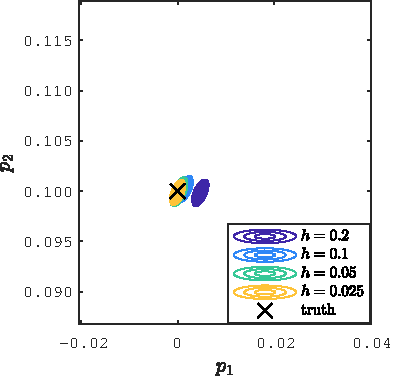
\includegraphics[]{BayesDet}
	\includegraphics[]{BayesDet2}
	\caption{$\pi^h_{\mathrm{det}}(y_0\mid y_{\mathrm{obs}})$, Störmer-Verlet}
	\label{fig:BayesB}
\end{subfigure}
\begin{subfigure}{\textwidth}
	\centering
	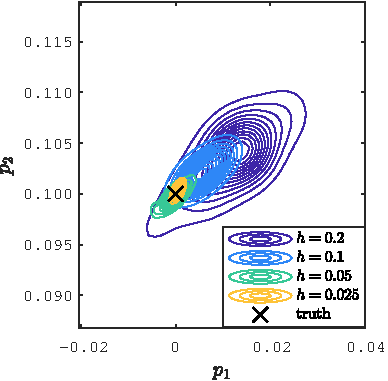
\includegraphics[]{BayesProb}
	\includegraphics[]{BayesProb2}
	\caption{$\pi^h_{\mathrm{prob}}(y_0\mid y_{\mathrm{obs}})$, RTS-RK Störmer-Verlet}
	\label{fig:BayesC}
\end{subfigure}
\caption{Deterministic posterior distribution for Heun's and Störmer-Verlet schemes and probabilistic posterior distribution for the RTS-RK Störmer-Verlet scheme for various values of the time step $h$.}
\label{fig:Bayes}
\end{figure}

\bibliographystyle{siam}
\bibliography{anmc}

\end{document}
